% brainstorm:

% * revisão das teorias de contornos
% * parte da análise que fiz do opus 5 mov 3 de Webern
% * exemplos de usos de operações na peça do mestrado e experimentos
% * desenvolvimento do goiaba (para que serve e um exemplo da saída)

\section{Introduction}
\label{sec:introduction}

Contours can be understood as the shape or format of an object. In
Music, they can be associated to elements like pitch, density, rhythm,
and represent a parameter in function of another, as pitch in function
of time. Contours can be easily recognized from graphic representation
by professionals and laymen alike \cite{marvin88:generalized}. For
instance, Beethoven's Fifth Symphony main motive and its pitch contour
are represented respectively in figures \ref{fig:5a-sinfonia-motivo}
and \ref{fig:c-3120}.

Contour is defined as an ordered set of distinct elements numbered
from the lowest to the highest \cite{morris93:directions}. In
contours, absolute values of its elements are ignored, and only the
high-low relationship between these elements is regarded. For
instance, figures \ref{fig:5a-sinfonia-motivo} and \ref{fig:ly-3120}
have the same pitch contour, represented in figure \ref{fig:c-3120},
and simbolicaly by (3 1 2 0).

The study of Contour is important because, like motives and pitch
sets, contours can help to give coherence to a musical piece. They
represent structural devices that can be combined through operations
like inversion and retrogradation, and can be aproached by analytical
or compositional points of view.

Systematic studies about the usage of contour operations and
combinations in musical composition are scarce, despite the possible
coherence that contours can give and the operations provided by
contour theories (see section \ref{sec:contour-theories}). Besides,
contour operations demand precise mathematical calculations and
graphical representations easy plotting. For these reasons, this
subject require more experimentation and studies about operations
usage in the field of composition, and a computer program to assist in
calculations and plotting, to avoid human errors and wasting time.

In this paper we present partial results of our
research\footnote{Additional information was omitted to keep
  anonymity, and will be included in final version.} about contour
applications in musical composition. We are developing a contour
processor software that receives as input symbollic contours and that
outputs symbolic and graphical representations of contours and
operations. Likewise, the first author of this paper, in his master's
research, composed a woodwind quintet based in contour theories
operations, and using the mentioned software (see section
\ref{sec:contour-composition}).

\section{Contour theories}
\label{sec:contour-theories}

Many authors
\cite{friedmann85:methodology,friedmann87:response,morris87:composition,morris93:directions,marvin.ea87:relating,marvin88:generalized,marvin.ea95:generalization,polansky.ea92:possible,quinn97:fuzzy,clifford95:contour,beard03:contour}
have developed theories to organize in a systematic way the knowledge
about contour. These theories were developed primarily as analytic
techniques for non-tonal compositions \cite{beard03:contour}, and
provide arrays, matrices and many operations to help the comparison of
contours, like inversion, translation, comparison matrix, and contour
interval array.

Music analysis under the point of view of contour have been effective
in tonal and non-tonal music. There are successful analysis of pieces
by A. Schoenberg \cite{friedmann85:methodology}, A. Webern
\cite{clifford95:contour}, L. Dallapicolla
\cite{marvin88:generalized}, and W. A. Mozart \cite{beard03:contour}
pieces. Clifford \cite{clifford95:contour}, for example, says contour
has a significant role in Webern pre-serial music structure.

\section{The usage of contour in Composition}
\label{sec:contour-composition}

The quintet mentioned in section \ref{sec:introduction} was composed
entirely using the contour processor software to simplify operations
and plotting. The piece is based on combinations of contour operations
associated to parameters such as pitch, tempo, density and
texture. This quintet is based on $\alpha$ six notes motive
(fig. \ref{fig:motivo-alfa}) and its derived contour P(5 3 4 1 2 0)
(fig. \ref{fig:c-534120}). This P contour, its subsets and
operations---retrogradation, inversion, rotation,
interpollation---were the only one used in the piece.

For instance, the tempo in this quintet---82, 66, 120, 108 and
112---have relations based in A(1 0 4 2 3) contour, a subset of P with
five elements. The number of instruments in piece first section, N(1 3
2 5 4), also are based in a P subset contour. The piece begins with a
solo, then a trio, a duo, a quintet, and finally a quartet.

Contour operations were also combined to produce new
material. Rotation were combinated with retrogradation, intervallic
expansion with interpolation, rotation with intervallic expansion, and
so on.

The contour software was essential to compose a \eng{fugato}, in the
quintet, because each piece of subject and countersubject were based
on different combinations of rotation and retrogradation operations.
The subject has original contour P(5 3 4 1 2 0) and factor 3 rotation
(fig. \ref{fig:sujeito-fugato}). Figure
\ref{fig:output-sujeito-fugato} has the contour software output for
graphical representations of these subject operations. Contoursubject
has original contour retrogradation repeated three times with
different rotation factors---5, 4 and 3
(fig. \ref{fig:contra-sujeito-fugato}). In the same way software
output for these operations are in figure
\ref{fig:output-contra-sujeito-fugato}.

Rotation and intervallic expansion occur like in figure
\ref{fig:notas-curtas-madeiras}. In flute the contour has original
form, and in clarinet there is a factor 2 rotation and an
expansion. In oboe there is a factor 3 rotation and contour deviation
justified by the gesture. In bassoon there is a factor 3 contour
rotation and retrogradation, and intervallic expansion.

\section{Conclusions}
\label{sec:conclusions}

Contour represented a significant structural device in cited quintet
compositional process. The majority structures of the piece were
composed based on contour operations. For this reason we believe
contour is as important to composition as to analysis.

The cited software has an important role in our research, automating
operations calculation and plotting. It can be very useful for
composition and analysis. In the future the software will also receive
as input scores in the Lilypond\footnote{\url{http://lilypond.org/}}
format and will have a graphical interface.
The next step in our research is to develop the software to provide a
better interaction with the user, and to compose short experiments to
test a larger operations corpus, and multiple layers contours, like
simultaneous association with pitch, duration, timbre and dynamics.

\break
%%% concentra figuras em um só lugar

\begin{figure}[!p]
  \centering
  \subfloat[Main motive]{
    \includegraphics{5a-sinfonia}
    \label{fig:5a-sinfonia-motivo}
  }
  \subfloat[Contour (3 1 2 0)]{
    \includegraphics{c-3120}
    \label{fig:c-3120}
  }

  \subfloat[Another (3 1 2 0) melody]{
    \includegraphics{ly-3120-qualquer}
    \label{fig:ly-3120}
  }
  \caption{Fifth Symphony main motive contour}
  \label{fig:5a-sinfonia}
\end{figure}

\begin{figure}[!p]
  \centering
  \subfloat[$\alpha$ motive]{
    \includegraphics{motivo-alfa}
    \label{fig:motivo-alfa}
  }
  \subfloat[P(5 3 4 1 2 0) contour]{
    \includegraphics{c-534120}
    \label{fig:c-534120}
  }
  \caption{Materials}
  \label{fig:materials}
\end{figure}

\begin{figure}
  \centering
  \subfloat[Subject]{
    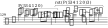
\includegraphics[scale=3.2]{sujeito-fugato}
    \label{fig:sujeito-fugato}
  }

  \subfloat[Countersubject]{
    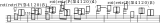
\includegraphics[scale=3.2]{contra-sujeito-fugato}
    \label{fig:contra-sujeito-fugato}
  }
  \caption{Structural elements of \eng{fugato}}
  \label{fig:elementos-fugato}
\end{figure}

\begin{figure}
  \centering
  \subfloat[Subject]{
    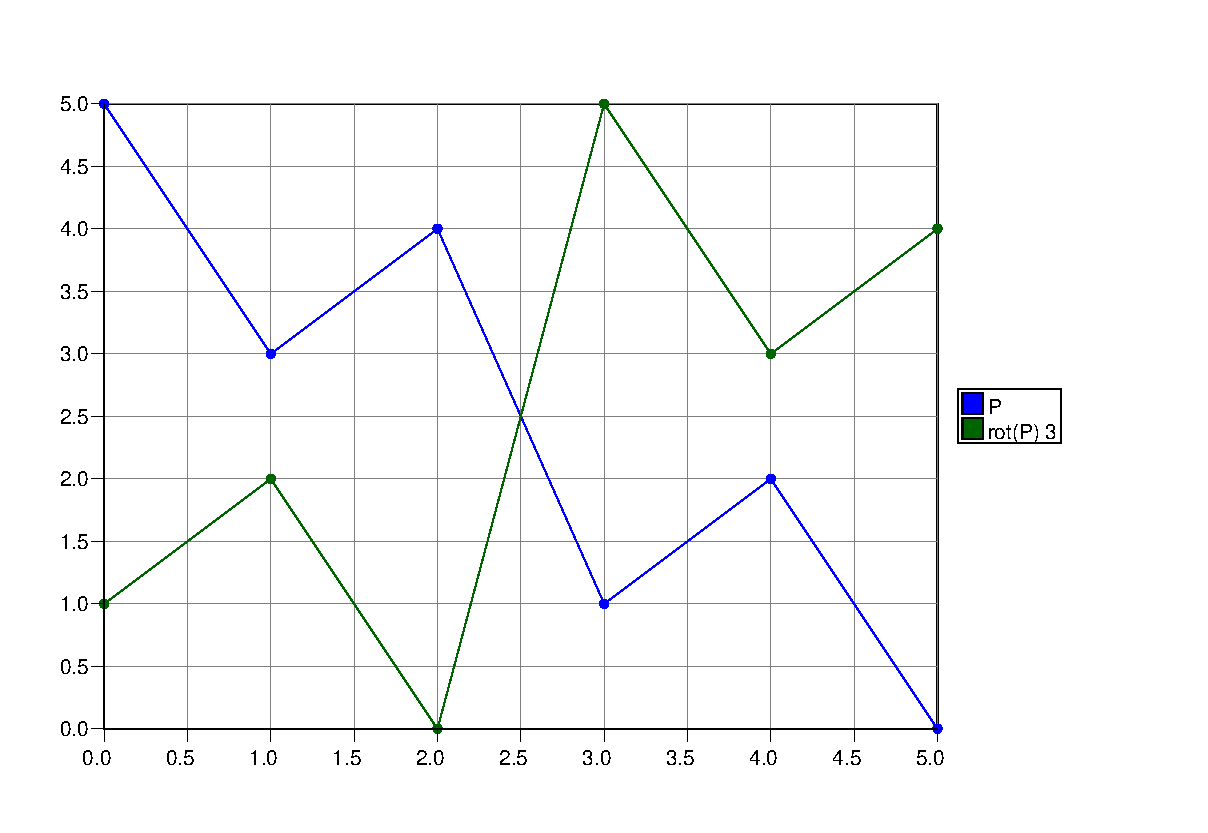
\includegraphics[scale=.44]{output-subject}
    \label{fig:output-sujeito-fugato}
  }

  \subfloat[Countersubject]{
    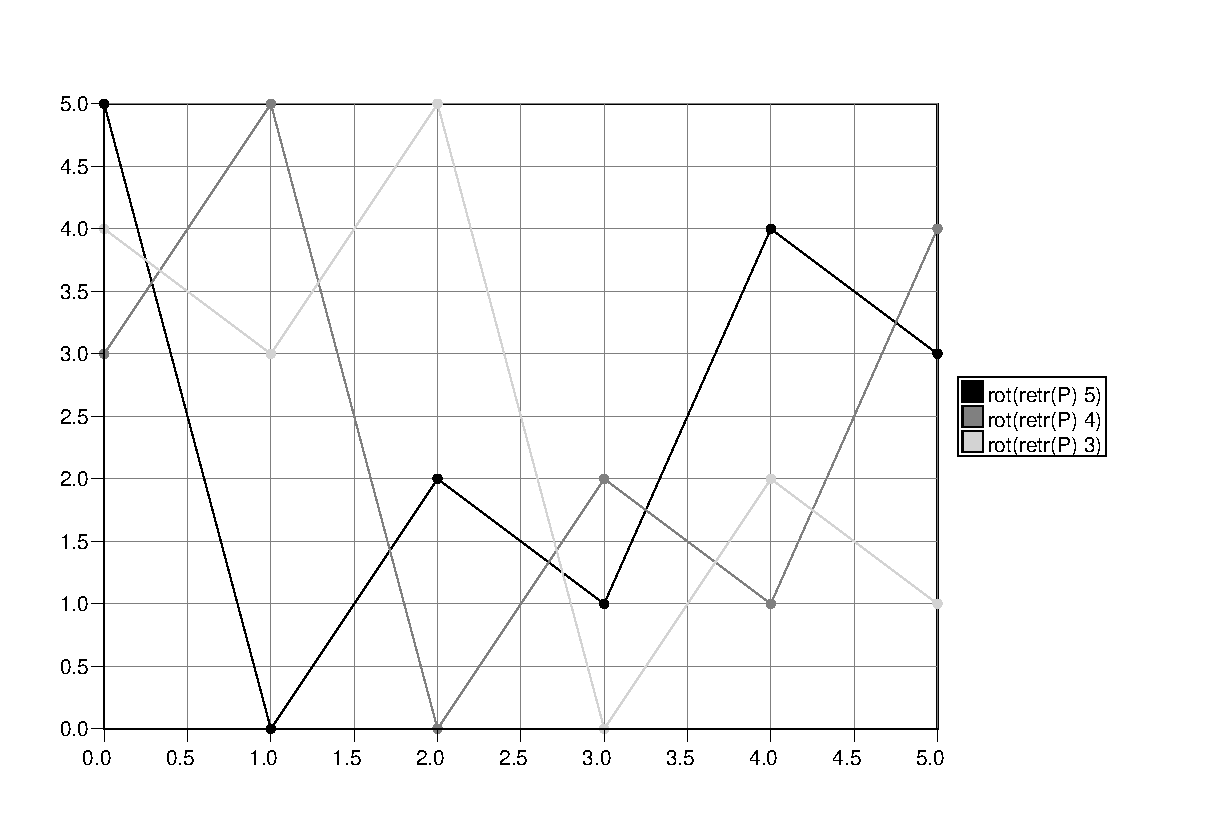
\includegraphics[scale=.44]{output-countersubject}
    \label{fig:output-contra-sujeito-fugato}
  }
  \caption{Software output for \eng{fugato} contour operations}
  \label{fig:output-fugato}
\end{figure}

\begin{figure}[!p]
  \centering
  \subfloat[4 fragments composed by rotation and expansion]{
    \includegraphics[scale=1]{notas-curtas-madeiras}
    \label{fig:notas-curtas-madeiras}
  }

  \subfloat[original]{
    \includegraphics[scale=.75]{c-534120}
    \label{fig:rot-0}
  }
  \subfloat[rot 2]{
    \includegraphics[scale=.75]{c-412053}
    \label{fig:rot-2}
  }
  \subfloat[rot 3]{
    \includegraphics[scale=.75]{c-120534}
    \label{fig:rot-3}
  }
  \subfloat[retr(rot 3)]{
    \includegraphics[scale=.75]{c-435021}
    \label{fig:rot-3-retr}
  }
  \caption{Rotation and expansion}
  \label{fig:rotacao-expansao}
\end{figure}

%%% Local Variables: 
%%% mode: latex
%%% TeX-master: "contour-composition"
%%% End: 